%%%       aums.sty (Masters Thesis)
%%%       auphd.sty (Ph.D. Dissertation)
%%%       auhonors.sty (Honors Scholar)

%%%To use it, please edit the necessary options, title, author, date, year, keywords, advisor, professor, etc. 

\documentclass[12pt]{report}
%\usepackage{aums}       % For Master's papers
\usepackage{auphd}     % Rodney edited the aums style to auphd
\usepackage{ulem}       % underlining on style-page; see \normalem below
\usepackage{url}
\usepackage{tikz}
\usepackage{pgf}
\usepackage{graphicx}
\graphicspath{ {./images} }
\usepackage{todonotes}
\usepackage{mathtext}
\usepackage{listings}
\usepackage{pgfgantt}
\usepackage{comment}
\usepackage{adjustbox}
\usepackage{outlines}
%\usepackage{natbib}
%%%%%Format rules: Normal margins are 1 in. If you need to print with 1.5in margins, uncomment the line below
%\oddsidemargin0.5in \textwidth6in

%% If you do not need a List of Abbreviations, then comment out the lines below and the \printnomenclature line.
%%for List of Abbreviations information:  (see http://www.mackichan.com/TECHTALK/509.htm  )
\usepackage[intoc]{nomencl}
\renewcommand{\nomname}{List of Abbreviations}   	       
\makenomenclature 
%% don't forget to run:   makeindex ausample.nlo -s nomencl.ist -o ausample.nls
%% Also, if 

% May want theorems numbered by chapter
\newtheorem{theorem}{Theorem}[chapter]

% Put the title, author, and date in. 
\title{Software Forensics for Adversarial Authorship}
\author{Rodney Visser} 
\date{Dec 17, 2020} %date of graduation
\copyrightyear{2020} %copyright year

\keywords{Software Forensics, Threat TTPs, Digital Provenance, Machine Learning, Recurrent Neural Networks, Convolutional Neural Networks, Threat Intelligence, Authorship Attribution}

% Put the Thesis Adviser here. 
\adviser{David Umphress}

% Put the committee here (including the adviser), one \professor for each. 
% The advisor must be first, and the dean of the graduate school must be last.
%\professor{David Umphress, Chair, Associate Professor of Computer Science and Software Engineering}
%\professor{James Cross, Professor of Computer Science and Software Engineering}
%\professor{Jeffrey Overbey, Assistant Professor of Computer Science and Software Engineering}
%\professor{Michael Hamilton, Assistant Professor of Electrical and Computer Engineering}

\begin{document}
\begin{romanpages}      % roman-numbered pages 
\TitlePage 

\begin{abstract} 
Software forensics in computer science can often used to determine intellectual property rights and it provides potential for threat attribution.  Risks from malicious software and the software supply chain are becoming more and more of an issue as code gets more complex and attackers continuously outpace defenders in the digital domain.  The software development process has changed significantly and threats have been on the bleeding edge of this maturity in terms of capability and obfuscation. The history and modern motivation for such analysis of software is present and includes commercial and government organizations.  This research looks at current static and dynamic methods of performing software forensics and improves on these methods by utilizing multi-dimensional analysis to detect semantic differences between two versions of a similar software code and then applying models in order to predict future changes in behavior.
\end{abstract}

%\begin{acknowledgments}
%Put text of the acknowledgments here.
%\end{acknowledgments}

\tableofcontents
\listoffigures
%\listoftables

\printnomenclature[0.5in] %used for the List of Abbreviations
\end{romanpages}        % All done with roman-numbered pages


\normalem       % Make italics the default for \em
%*********************************************************************
%*********************************************************************
%Chapter One (CH1)
%*********************************************************************
%*********************************************************************
\chapter{Introduction}  
\label{chap:one}

A quickly growing use case of software forensics is authorship attribution, the process of attempting to identify the likely authorship of a software sample given a collection of software whose authorship is known.  Convention points to the use of a subfield of digital forensics, software forensics,  to apply authorial context to the providence of malicious software.  The categorization and mapping of key properties extracted from a suspect artifact can be used to select candidate matches from a pool of legitimate artifacts.  We aim to provide a glimpse into the genealogy of a malware sample through the lens of software forensics.

Currently, reverse engineering software artifacts suspected of being malicious code remains a labor-intensive and manual task, despite advances in automated programming understanding.  Static and dynamic analysis tools provide insight into software structure and behavior, but the ultimate determination of what is a malicious artifact relies heavily on the skills and experiences of individual forensic investigators.  Further complacating the process, attackers have also begun to place false flags within the technical breadcrumbs that are commonly left behind after a cyber attack.  

A cost effective example of malware delivery method is through the use of phishing emails, where the content of the email tries to entice the recipient to click a URL linking to a malicious web site or downloading a malicious attachment. Analysts attempting to provide intelligence on such activities quickly find that the ever increasing volume of phishing emails circulating daily is overwhelming and the most effective phishing techniques are often not caught because of their use of the proper application of backstopping.  Therefore, intelligence gathered within this area is only representative of only a small sample at a single point in time, not of the global picture of the problem.  Additionally, analyses have revealed that authorship attribution analysis on this type of malware delivery method have provided linkages to the same author within clusters were likely, but that it is unlikely that the authorship-based clustering algorithms have managed to group together all spam produced by each group.  This problem of high precision with low recall, has been faced in past authorship research \cite{li2017association}.  In broader terms, the issue of authorship attribution of malicious code suffers from the same issues, but is further complicated by the variety of multi-dimensional inputs.  Examples of these inputs are delivery methods, obfuscation, and placement of false flags.

One of the most dangerous trends in authorship attribution for cyber attacks is the lack of specific knowledge about technical capabilities, motivation, policies, and laws that currently govern this area.  The difficult technical side of attribution is further escalated by serious legal and policy questions about when and how to accuse governments of responsibility for cyber attacks.  Within the area of technical capabilities and motivations for groups that have been labeled as Advanced Persistent Threats (APT)s by commercial cyber security firms, there are sweeping differences in the arrangement, categorization, and number of named threats from nation states or criminal enterprises. \cite{romanosky2019private}

\begin{table}[h!]
  \centering
    \caption{Named APTs}
    \label{tab:table1}
    \begin{adjustbox}{width=\textwidth}
    \begin{tabular}{l|c|c|c|c|c} % <-- Alignments: 1st column left, 2nd middle and 3rd right, with vertical lines in between
      \textbf{Country} & \textbf{FireEye} & \textbf{CrowdStrike}  & \textbf{Kaspersky} & \textbf{Dell SecureWorks}  & \textbf{Cisco Talos}\\
      \hline
      China & 20 & 40 & N/A & 5 & 9 \\
      Russia & 3 & 3 & N/A & 6 & 3 \\
      Iran & 3 & 7 & N/A & 1 & 3 \\
      North Korea & 1 & 4 & N/A & 2 & 2 \\
      Criminal / Terrorist & 10 & 29 & N/A & 3 & 1 \\
      Other & 2 & 1 & N/A & 2 & - \\ 
      Unknown/Undisclosed & 8 & 1 & N/A & - & 1 \\
      \hline
      Total & 47 & 85 & 36 & 19 & 19\\
    \end{tabular}
  \end{center}
\end{table}

Although politics may largely determine whether attributions are made public, there is a need for a framework in which when cyber attacks are attributed to states in a means governed by legal standards \cite{eichensehr2020law}.  Experts on the topic of cyber threat attribution are quick to call for greater levels of regulation and policy that govern the world's critical infrastructure and economies, but for the most part, worldwide leaders in key positions do not understand the issues presented to them, the proper information is not made available, or the terrain of navigating the geopolitical landscape on this issue in the public eye in deemed risky.

A prime example of state sponsored cyber espionage and influence operations is the unauthorized access and disclosure of the Democratic party's email in 2016 by a Russian State backed hacker group commonly referred to as Fancy Bear.  The main point of communication for this operations was a self proclaimed Romanian hacker called Guccifer 2.0.  Toni Gidwani, director of research operations for ThreatConnect, said: ``It would suggest to us that the operators of the Guccifer 2.0 persona were not the actors who breached the DNC.  You’re looking at the operations guys who don’t have the same technical credibility as these very sophisticated actors who exploited these networks. You've got a lot of cooks in this kitchen here, not just one actor.'' \cite{zager2016response}

This type of misdirection campaign for state sponsored hacking is considered common place now and automated single-dimension attribution techniques are easily guided into the wrong direction.
There are examples of two recent applications of technology within the realm of source code authorship attribution methods with accuracy above 88\%, but successful adversarial learning attack methods have been demonstrated that drops their rates of attribution to around 1\% \cite{abuhamad2018large}, \cite{caliskan2015anonymizing}, \cite{quiring2019misleading}. 

For these reasons, attribution must be thought of as a multi-dimensional issue that draws on multiple sources of information available, including technical forensics, human intelligence, signals intelligence, history, and geopolitics, among others \cite{lin2016attribution}.  If successful, the attribution of successful adversarial attacks from code left behind on an infected system could enable software forensics to be leveraged in order to be fight advancing and evolving threats. 

\begin{comment}
Why it is important 
    - expert opinions - if only we could apply attribution
	    2016 presidential election
	    Olymipics hack (Wired)
	    Sony hack

    - number statistics
        attack has a substantial effect on two recent attribution methods,  whose accuracy drops from over 88 percent to 1 percent under attack.
    
        [1] M. Abuhamad, T. AbuHmed, A. Mohaisen, and D. Nyang. Large-scale and language-oblivious code authorship identification. In Proc. of ACM Conference on Computer and Communications Security (CCS), 2018.
@inproceedings{abuhamad2018large}

        [9] A. Caliskan, R. Harang, A. Liu, A. Narayanan, C. R. Voss, F. Yamaguchi, and R. Greenstadt. Deanonymizing programmers via code stylometry. In Proc. of USENIX Security Symposium, 2015.
@inproceedings{caliskan2015anonymizing}

	DU "I don't get a scense of the degree to which the problem is relevant.  Please provide information which points to the impoertance of solving the problem.  Substantiate with facts."

A. INSERT Ref to "ODNI_A_Guide_to_Cyber_Attribution"
"Establishing attribution for cyber operations is difficult but not impossible.  No simple technical process or automated solution for determining responsibility for cyber operations exists.  The painstaking work in many cases requires weeks or months of analyzing intelligence and forensics to assess culpability.  In some instances, the IC can establish cyber attribution within hours of an incident but the accuracy and confidence of the attribution will vary depending on available data."


Addin Bruce Scnider reference on threat attribution and one from ex-Microsoft Executive that was the Cyber Czar and incorrect about China." Howard Anthony Schmidt died in 2017 at the age of 67

E G See, Rt, Philip Hon, Hammond
I unequivocally condemn these cyber attacks [on Sony] and am deeply concerned at the findings of the US investigation, which seems to provide further evidence of North Korea's blatant disregard for international norms and obligations
Foreign & Commonwealth Off
Posted: 2014-12-19

E G See, Bruce Schneier
I am deeply skeptical of the FBI's announcement on Friday that North Korea was behind last month's Sony hack. The agency's evidence is tenuous, and I have a hard time believing it
Posted: 2014-12-22

E G See, Jack Goldsmith
sony-hack-attribution-problemsand-connection-domestic-surveillance (noting that "the 'evidence' is of the most conclusory nature" and "on its face . . . shows only that this attack has characteristics of prior attacks attributed to North Korea
Posted: 2014-12-19
\end{comment}

\section{Software Forensics}
  The history of software forensics is a relatively brief one when compared to other forensic sciences.  It began with methods for finding similarities in software by comparing code through hashing, statistical analysis, text matching, and tokenization.  These methods compared software code at a primitive level by ingesting sources and producing a single measure indicating similarity.  These measures were not accurate enough to be admissible in modern courts because the algorithms used to find them could be easily fooled by simple substitutions.  ``The discipline of computer forensics appears to be struggling over methods and practices that will meet the courts’ “standards” for scientific evidence" \cite{meyers2005digital}.

By first examining similarity of a software artifact to other artifacts that have been previously observed, investigators can frame deeper questions, such as investigating new or changed capabilities.  For example, clues as seemingly insignificant as the format of calendar dates or the language used in text strings can be used to help identify demographic origins.  Level of sophistication, control flow patterns, stylistic flourishes, obfuscation techniques, and unique defects have the potential to signal the education and skill level of an artifacts creator or creators perhaps going so far as to call out our artifact authorship given a collection of samples from a known author or authors.  Indirect information of this type, if available and used properly, offers a context so that investigators are not working in a vacuum, where each suspect artifact has been treated as a never before seen item.

The challenge becomes one of how to automate the use of attributes as figurative fingerprints capable of leading software forensic investigators to artifact lineage and pedigree.  Principal unresolved issues include how to identify which attributes determined similarity among artifacts, how to assess the trust of information inferred from the use of attributes, and how to establish unreliable enough approach to satisfy legal standards.

\section{Problem Statement}
\label{sec:ProbState}
Within the questions of \emph{what, when, where, who, and how} for digital forensic investigations, answering the question is frequently the most elusive.  The strategic aim of this research is to assist in answering this important question.  The tactical objectives include a survey of current state-of-the-art techniques in adversarial authorship using software forensics and the application of machine learning to automate and innovate analysis.

Software-assisted detection allows vast collections of artifacts to be compared to each other, making successful detection much more likely than traditional manual methods.  We refer to these first generation software-assisted means of detection as Single Dimensional Software Correlation.  This method can be thwarted by simple compiler optimizations and anti-forensic techniques.  Differences in hashing and mapping methods can cause a significant increase in false negatives count.

The motivation to use more focused and robust software forensic techniques is growing at an expanded rate in order to keep up with the adversarial techniques malware authors use to obfuscate their code.  Cyber threat actors for the most part are out pacing the defenders at an increasing rate, modern software forensics tools, techniques, and procedures are growing, but not fast enough to lessen the gap with threats.  In order to keep pace with intermediate and advanced level threat actors, novel techniques must be employed to find, track, and project how threats are evolving.  Adversarial authorship using software forensics can allow us to do this.

%********************************************************************
%********************************************************************
%Chapter Two (CH2)
%********************************************************************
%********************************************************************
\chapter{Literature Survey}
\label{chap:two}
Using software forensics to track and plot the actions and potential growth of cyber threat actors includes problematic factors such as: lowered barriers of entry in terms of technical competence, malware as a service platforms, increasing levels of sophistication, and an rapidly expanding attack surface.  The development of a novel graph pruning technique has shown that software correlation can be used to understand how malicious code has evolved over the years, and in particular, how different instances of malicious code relate to one another.  Researchers established an inheritance relationships between different instances of malware based on temporal information and key common phrases identified in the malware descriptions and an extension of this research has the potential to show that software correlation can be used to inspect known examples of malware in order to gauge how threats and their code bases are evolving \cite{gupta2009empirical}.

Authorship attribution has its roots in plagiarism detection, which is the process of locating instances of literary theft within traditional documents.  The word \emph{plagiarism} dates back to the first century AD with the Roman poet Martial, one of the most prominent poets of his time.  Martial discovered that his work was being copied and provided wholesale without proper attribution.  Unlike other authors in a similar predicament at the time, Martial was not content to stand by and other take credit for his work.  He wrote several verses directed to his copycats.  One in particular was aimed at a man named Fidentinus \cite{martial:1958}:

\begin{quote}
``FAME HAS IT THAT YOU, FIDENTINUS, RECITE MY BOOKS TO THE CROWD AS IF NONE OTHER THAN YOUR OWN.
IF YOU’RE WILLING THAT THEY BE CALLED MINE, I’LL SEND YOU THE POEMS FOR FREE.
IF YOU WANT THEM TO BE CALLED YOURS, BUY THIS ONE, SO THAT THEY WON’T BE MINE." 
\end{quote}

In one of his poems he used the latin word \emph{plagiarus} to describe a literary thief.  In his time the term meant to kidnap, and it specifically related to either the kidnapping of one's slaves or to take a free person and make them into a slave.

The modern day widespread use of computers connected to the Internet has eased the task of the plagiarist.  A great deal of cases of plagiarism can be found in academia, where documents are typically essays or reports, but plagiarism can be found in virtually any field, including software engineering. \cite{!stealsc:2012}

In the case of software plagiarism, advanced obfuscation techniques have made automated detection at scale increasingly difficult because of the ease of change in the structure of the code while preserving the code semantics \cite{xu2020revisiting}.  As an example, setting within software compilers can easily configured to be used as a obfuscation techniques to change the assembly code, resulting in a low similarity score.  For prototypes that have been seen to be resiliency to advanced code obfuscation, there is a problem of scale.  Most graph-based approaches are time consuming since it is a NP-hard problem.  Within an example of semantics-based approach using graphs, it took an hour in  the  comparison \emph{thttpd} and \emph{sthttpd}, and half a day in the comparison between \emph{Gecko} and \emph{Firefox} \cite{luo2014semantics}.  Given the rate of increase at which malicious programs are being created with the application of advanced obfuscation techniques, the scalability to process samples becomes a critical need.

\begin{comment}
DU "I have a tough time understanding the link between plagiarism and author attribution.  Plagiarism is demonstrated by proving that a suspect artifact sufficiently resembles any other artifact.  It does not imply that we can not infer knowledge about the artifact based on the original source.  I think you need to tighten your chain of logic in linking plagiarism to authorship attribution...or eliminate the plagiarism piece altogether.

	DU "Plagiarism = the suspect artifact is a copy of something else
	    You want = Who is the originator and, if we have seen it before, what do we know about the original"

	plagiarism section - where is the original source
		* link with technical example of an attribution problem

	Sandworm - Andy Greenberg Wired Magazine - 2018 Olympics Russian Cyber Attack - South Korea
		Miss-direction using false flags

Here is how attributions done and how can we do it better?
\end{comment}

\begin{comment}
STUXNET - why is authorship attribution of 2 nation states working together to on a important project important
		more history on the attribution side
			(why is authorship attribution ***ch.1*** )

	DU "I don't see where you describe how stuxnet was understood because of its origins were traced to an original.  In other words, I did not see a plagiarism or an authorship attribution aspect in this description."
\end{comment}

The devastating cyber attack referred to as the NotPetya worm is example of the greater levels of need for advancing software forensic tools in order to better help determining adversarial attribution.  The NotPetya worm was created by a group of Russian military intelligence hackers known as Sandworm, and was intended as a climactic strike against Ukraine in the years-long cyberwar Russia had carried out against its southwestern neighbor.  This worm presents an interesting case because of the unique combination of using stolen National Security Agency hacking capabilities, an open-source credential-harvesting tool called \emph{Mimikatz}, and the hijacking of a update system within a common piece of Ukrainian accounting software that was used used by practically every company that filed taxes or had business ties in the country.

\begin{comment}
Shadow Brokers, EternalBlue, EternalRomance
    ETERNALROMANCE is a SMB1 exploit over TCP port 445 which targets XP, 2003, Vista, 7, Windows 8, 2008, 2008 R2, and gives SYSTEM privileges (MS17-010)
    ETERNALBLUE is a SMBv2 exploit for Windows 7 SP1 (MS17-010)

WannaCry ransomware used this exploit to attack unpatched computers.
\end{comment}

\begin{comment}
The Stuxnet worm is an example of the greater levels of need for advancing software forensic tools in determining adversarial attribution. \cite{parker2011stuxnet}  One area of Stuxnet was the use of a modified Step7 library file, named s7otbxdx.dll, to communicate with a Siemens Programmable Logic Controller (PLC) (see Figure \ref{fig:stuxnet-modified-s7otbxdx.dll}).  

\begin{figure}
	\centering
	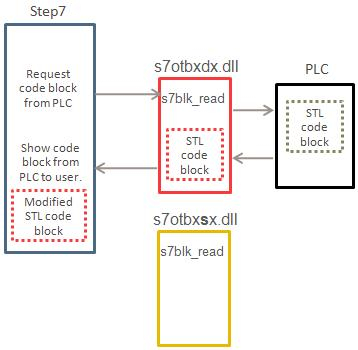
\includegraphics[width=0.5\textwidth]{images/modified_Step7.jpg}
	\caption{Stuxnet’s modified s7otbxdx.dll file \protect\cite{falliere2010exploring}}
	\label{fig:stuxnet-modified-s7otbxdx.dll}
\end{figure}

Stuxnet's modified s7otbxdx.dll forwards 93 of the original 109 exports to the real DLL, renamed to s7otbxsx.dll, for processing.  16 exports were intercepted by the custom DLL in order to modify data being sent to or returned from the PLC without the operator of the PLC realizing it. It is also through these routines that Stuxnet was able to hide malicious code on the PLC itself.
\end{comment}

In order to use software forensics to track advancing threats like that of NotPetya, the software forensics engineer needs to break the inputs into objects suitable for comparison and apply structure to these objects.  This structure can then be used to determine which objects exist across various versions and which do not.  This is not a simple task since the differences in high-level language constructs and structure, including code comments, are commonly not found in the compiled versions of the malicious software.  Techniques used to identify commonalities are single and multidimensional software correlation. 

\section{Single Dimensional Software Correlation}
Single Dimensional Software Correlation takes a single input source and uses that source to apply structured analysis.  This analysis determines the similarity of source or binary code, by comparing their raw text, cryptographic hashes, and tokens.  The result is a single measure that indicates the degree of similarity.  These measures are not accurate enough to be admissible in court of law because they are not definitive.  Questions arise because the algorithms can be fooled by, for example simple substitutions in the code with representative fixes.  As a case in this point, the problem of instruction reordering can be solved though grouping using the variable tracing and sorting method \cite{oh2009fight}.

\cite{zeidman2012detecting} developed algorithms that look at the basic elements of code in order to find which elements are correlated to each other.  He proposed an algorithmic method that extracts program elements that are common in the samples being compared.  These methods keep each of the data structures that are found to have entries corresponding to program elements of a distinct program element type represented by program strings or program identifiers.   From that, elements are extracted based on a program object code file using a text converter to convert the program object code to text sequences by solely determining byte by byte whether the sequences represent characters.  Then a calculation of a correlation score based on the similar entries is done that is comprised of a number of similar strings and a number of similar identifiers.

\begin{comment}
The major drawback to this work is the high number of false positives that result from the comparison.  Efforts to improve accuracy included interpreting the elements being compared to eliminate reasons for correlation unrelated to copying, such as common algorithms, third-party code, common identifier names, common author, and automatic code generation.

DU Comment = citation(s) needed
\end{comment}

Another single dimensional software correlation technique is analysis of code comments.  Once analysis has been performed using single dimension software forensic tool and/or procedure, an analyst can then begin looking at subjective evidence such as comments in the code.  Fake copyright notices, open source notifications, or programmer names added to source code after copying took place, in order to disguise the copying, are not uncommon in real-world cases of code theft \cite{sfbook:2011}.  This has been shown in practice to support a number of different challenges and benefits.  Challenges arise in the ways that code comments are written using natural language, which make these comments difficult for a computer to automatically understand the intent of the comment even when armed with the latest Natural Language Processing (NLP) techniques.  \cite{artsci:2015}  As a benefit, code comments contain a rich amount of information that can be leveraged to improve attribution.  Analyzing free-form and semi-structured code comments can assist in the unique identification of characteristics and content of code comments.

The value of code comment analysis is improved when presented with strong pieces of supplemental data.  Information such as how an organization distributes its code, details of the software development life-cycle can possibly emerge.  This gives the potential to identify the programmers who authored the code.  

There is also work being done on data sets of different programming languages (Java or C++) of varying difficulty (6 to 30 candidate authors) to demonstrate the effectiveness of the Source Code Author Profiles (SCAP) approach.  This is based on analysis of byte-level contiguous sequence profiles in order to represent a source code author’s style.  \cite{IFIP:2006} This method has potential to show effectiveness of the model and how it is not severely affected by the absence of comments in the source code, a condition usually met in cyber-crime cases.

The analysis of malicious code authorship and true functionality without the assistance of the underlying source code makes single dimensional software correlation difficult and a prime target for deception.  Comparing code functionality is a difficult problem that has yet to be effectively shown by any algorithm within a reasonable time.  For this reason, the process of applying attribution to a code's author is still mostly manual.

\section{Multidimensional Software Correlation}
Multidimensional software correlation is the process of dividing software code into separate parts in order to determine which elements are similar.  One of the key elements to applying this correlation is the ability to filter and/or interpret the correlations in order to eliminate false positives.  The state of research of semantic data models being leveraged for machine learning has shown promise in helping identifying similar elements for correlation.  One example of this work is the concept of traceability being applied using machine learning within safety-critical domains for source code and other artifacts.  It uses Word Embedding and Recurrent Neural Network (RNN) models to generate trace links.  RNN models use these word vectors to learn the sentence semantics of requirements artifacts.  From that the analysis can be used to learn the semantic word vectors that represent knowledge of the domain.  An RNN system that uses Bidirectional Gated Recurrent Units (BI-GRU) has shown promise for the tracing task.  BI-GRU, in this instance significantly out-performed state-of-the-art tracing methods including the Vector Space Model and Latent Semantic Indexing.  \cite{guo2017semantically}

An important piece of addressing attribution using software correlation is the transit data path, means, and capabilities.  There is promising research being done within the area of time-series forecasting methods for cyber attacks, from network telescopes, honeypots, and automated intrusion detection/prevention systems.
This is limited to awareness of predesignated items within a temporal scope that can be easy to miss and hard to collect.  ``To enhance awareness about specific threats, it is vital to uncover associated and, ideally, causal factors for cyber attacks"  \cite{DBLP:journals/corr/BakdashHZMTSHD17}.  For our research endeavor, this data can be used to assist in attribution based on past observation of transit data path, means, and capabilities.  These supporting factors can be used in order to further judge breadth, depth, and positioning of future attacks in traditional and new environments that threats are working towards having similar capabilities that exist in client-server environments.

Provenance, a word that originates from art, refers to the chronology of location and ownership.  A detailed provenance can be used to establish that a piece of art is not a forgery, or has not been stolen.  Recently, the term provenance has also been adopted and applied to other fields, including computer science, where it refers to having knowledge of all the steps involved in producing a scientific result, from experiment design through acquisition of raw data and all the subsequent steps of data selection, analysis, and visualization \cite{provenance:2011}.

The concept of provenance can also be applied to multidimensional software correlation.  The tracing of provenance in software development has become increasingly more important to tracking vulnerabilities and threats.  Models of provenance developed from observing software during its natural life cycle can be used to educate researchers on how code evolves and mutates over time.  The relation between a large file and LOC objects is very sparse and indexing can allow the relations to mapped as clusters of LOC and their containing files.  Using these observations an analyst is able to observe statistical trends of modifications made to files over time and see changes in sparse structures and natural growth patterns throughout a software development life cycle.  In a typical scenario, files exhibit rapid initial growth with code being added in large chunks, and then when the changes of the software are in place, small bug fixes are the majority of modifications there after.  By tracking the unique relationship between file size and lines of code, an analyst map codelets as code patches with co-migratory patterns in files.  \cite{provenance2:2014}  For instance, a generative model that uses a Bayesian game to assist in Active Malware Analysis (AMA) has shown to have strong statistical results in identifying relations in software provenance between malware families \cite{sartea2020bayesian}.  

Traditional grammar-based analysis techniques used to detect plagiarism have been adapted for use in code source plagiarism detection \cite{kustanto2009automatic}, \cite{lesner2010novel}, and \cite{jadalla2008pde4java}.  Code, like speech, consists of patterns that can link the author to the product.  Prolog offers advantages for a thorough analysis in two main parts.  In one part, it natively provides versatile options to efficiently process tree or graph data structures.   In another part, Prolog’s non-determinism and backtracking eases tests of different variations of the program flow without a large level of effort.  A rule-based approach with Prolog allows to characterize the verification goals in a concise and declarative way.  This is why the Prolog programming language is currently being used to do source code verification for embedded aerospace systems \cite{flederer2017source}.  

Multidimensional software correlation can be leveraged in order to collectively analyze more data inputs that single dimensional Software Correlation, but this does not necessarily mean that the results will be more useful or efficient.  Issue exist in the accuracy of the data gained, but on a grander scale because of the increase in the number of inputs.  In terms of efficiency, there are also issues in terms of computing and analyst time required to get though the raw data and explore the results to find the applicable truths.  

\begin{comment}
A common technique to verify programs of a safety critical nature is the analysis of their Abstract Syntax Tree (AST).  Tree structures can be analyzed with the logic programming language Prolog.

\section{Deep Neural Networks}


DU "I'm not sure this section is needed, unless you plan ot advance the state-of-the-art in nural nets.

Authorship attrubution is done in the way today "Single Correlation and Mutiple Correlation...

xyz - smith uses mutiple correlation though hyper regression means or neural network
	more examples
	why using NNets vs traiditional statisitical means
	pros and cons


There are many different combinations of ways to implement inventions in software and even the most powerful of modern computers cannot consider all combinations of how that code might infringe on a patent or identify the original author because of inherent complexity.  This work is still left to human experts using their knowledge and experience and similar to that of factual based evidence research, much of the same highly knowledgeable and experienced skill sets cannot be easily taught or automated. \cite{influence:2009}  This is a problem that many in software forensics are trying to automate by finding an algorithm or simplifying process, but it has not proved to be an easy task.

Deep neural networks (DNN) is a means by which multiple layers between the input and output can be applied in order to model complex non-linear relationships.  For this proposal the aim is to apply this type of analysis in order to speed up the time in which it would normally take an analyst to find/evaluate reliable indicators of malicious software intent, which cutting down on the high false positive rates of traditional single and multidimensional software correlation.  In order to do this, vectors that are expressed as constant maps will be concatenated into sets of weighted layers.  During the training process, the application of the various natural language processing indicators for malicious intent can be used as a parameter that can also updated by backpropagation.  A similar application of neural networks is being applied to software defect prediction in order to show significant improvement over baseline techniques \cite{phan2018convolutional}.

\subsection{Recurrent Neural Network}
A recurrent neural network (RNN) is a specific class of deep neural network where the connections between units can form a directed graph along a sequence that allows analysis for dynamic temporal behavior for a time sequence.  Research has shown that an ensemble of recurrent neural networks are able to predict whether an executable is malicious or benign within the first 5 seconds of execution with 94\% accuracy \cite{rhode2017early}.  Adversarial authorship was not a focus point for this research, but some of the concepts could be used provide a temporal based analysis of the authorship problem.

\subsection{Convolutional Neural Network}
A convolutional neural network (CNN) is a specific class of deep neural network where the network is made up of neurons that have weights and biases.  Within this, each neuron receives some inputs, performs a product and optionally follows it with a non-linearity.  The whole network still expresses a single differentiable score function, an example would be from the raw image pixels on one end to apply class scores at the other end.
\end{comment}

\section{Summary}
All single dimensional software correlation techniques have in inherent weaknesses within the application of authorship attribution for malicious software.  The state of the science needs to be provided a framework of multi-dimensional software correlation that can help spread the sources of attribution across areas of analysis in order to better apply augmented intelligence and allow analysts to navigate the maze of false positives.  

\begin{comment}
DU's resposse to part of your summary 'All software correlation techniques share a weaknesses of difficult in determining is the correct input or inputs being analyzed and is it from a trustworthy source.' = "huh?"

DU comments onlast sentence "ok...so what does this have to do with you?  Need a logical connection to your proposal solution"
\end{comment}

%**********************************************************************
%**********************************************************************
%Chapter Three (CH3)
%**********************************************************************
%**********************************************************************
\chapter{Proposed Solution}
\label{chap:three}
This research proposes applying the multidimensional software correlation concepts with the assistance and extension of the Lockheed Martin Cyber Kill Chain \cite{hutchins2011intelligence}, MITRE ATT&CK framework \cite{strom2018mitre}, and National Vulnerability Database (NVD) \cite{zhang2011empirical}.    

The Lockheed Martin Cyber Kill Chain allows analysis to happen at different stages with the natural cycle of a cyber attack without having to start from the beginning.  This is important because of the increased use of separate teams for areas of specialty that support the same mission.  Additionally, the state of digital security is such that most intermediate and advanced cyber threat actors are not found to have compromised a system for an extended period of time from when reconnaissance started.  There are the seven steps of the Cyber Kill Chain: Reconnaissance, Weaponization, Delivery, Exploitation, Installation, Command and Control (C2), and Actions on Objectives \cite{martin2014cyber}.

``The MITRE ATT&CK knowledgebase describes cyber adversary behavior and provides a common taxonomy for both offense and defense. It has become a useful tool across many cyber security disciplines to convey threat intelligence, perform testing through red teaming or adversary emulation, and improve network and system defenses against intrusions"  \cite{strom2018mitre}.   This framework can also be used to assist in the application of providence for the tactics and techniques to be define as adversarial behaviors within a lifecycle to a degree where they can be more effectively mapped to attribution. 

The National Vulnerability Database (NVD) is a synchronized and search-able database of publicly disclosed cybersecurity vulnerabilities and exposures \cite{NIST_NVD:2020}.  The NVD consists of Common Vulnerabilities and Exposures (CVE) entries and is extended to include additional data such as fix information, severity scores, and impact ratings. As part of its enhanced information, NVD also provides advanced searching features such as by OS; by vendor name, product name, and/or version number; and by vulnerability type, severity, related exploit range, and impact.

We propose applying multidimensional software correlation to help better track and identify behavior changes in malicious software artifacts and authors.  Using forensic software analysis to determine the function and motivation between malicious software examples can allow for the syntactic differences in implementations to be discarded, but be able to focus on the program's mapped semantic characteristics to determine origin and a potential future path.

\section{Research Goals}
The primary goal of this research is to apply augmented intelligence techniques based on validated cyber threat intelligence and leverage the combined frameworks to enable forensic software analysis to better determine the linage of malicious software threats.  A secondary goal of this research is to explore the areas of analyzing current and projecting future complexity of malicious software in non-standard environments.

***
\begin{comment}
DU comment on research goals "I don't know what this says" = 'map semantic data models in order to determine the linage of malicious software.'  Also, what does 'non-standard environments' "mean?"
	Map data models to apply?

What is the major contribution?  What is the CS link to changing the world?
\end{comment}

\section{Research Idea}
The novelty of this research is in first, determining the role authorship plays in the similarity factor of software artifacts, and second, projecting the trajectory of of behavior based on the providence of artifacts attributed to a specific author.  When black box analysis of a particular software's attributes (syntax, functions, inputs, return values, and comments) are done to map relations between known identifiers.  If similar attributes are found from two different examples then similarities will be drawn between their behavior.  The same black box analysis will also be applied over a large pool of malicious software examples in order to find trends in currently known capabilities and future focus areas.  The strength of these methods used together will be leveraged in order to augment traditional techniques in software forensics to more accurately identify and project the trajectory of malware. 

We plan to tailor the research to cyber threat actors with known characteristics by first linking actions and tools that fall within the framework to a signature of mapped attributes in order to determine providence and provide further matches or changes within these characteristics.  This idea is similar to how \cite{oh2009fight} used variable-length fingerprints across a series of instructions to describe how data is used within a function or basic block.  The order and path of data transformations are important and uniquely identifiable, such as in the same way that an mystery author's work can be identified because of key characteristics.  

\begin{comment}
DU comments on last paraphgraph within 'Research Idea' = "while this is a good 100k-foot descroption, we need a more deailed explanation"

	DU = Change reference display from '[Oh 2009]' to "Oh [2009]"
\end{comment}

\section{Research Hypothesis} 
The research hypothesis is ``the software correlation mapping technique will be 92\% more accurate than current active malware analysis methods''. The null hypothesis this research will seek to disprove is ``the software correlation mapping technique will preform equal to or worse than current active malware analysis methods''.

\begin{comment}

DU "think of a hypothesis as being a metric by which you will know when you are done.  Consider phrasing the hypothesis in measuable terms.  Also section 3.2 suggests you have two hypothesises"

	Change your research hypothisis
		state your requirement as a yes or no
		what signture based techniquences

		research plan - current validation section Pytorch and Tensor Flow
		null hypothsis - will not preform any better than the current state of the art
\end{comment}

\section{Validation}

\subsection{Validation Outline}

\begin{outline}[enumerate]
\let\OldOne\1%
\let\OldTwo\2%
\let\OldThree\3%
\renewcommand*{\1}{\normalsize\normalfont\OldOne\bfseries\Large\scshape}%
\renewcommand*{\2}{\normalsize\normalfont\OldTwo\bfseries}%
\renewcommand*{\3}{\normalsize\normalfont\OldThree\small}%
\1 Setup system to analyze malware in datasets A and B
    \2 Collect software's attributes from dataset A, then B
        \3 syntax, functions, inputs, outputs, return values, comments, etc
    \2 Apply 3 level framework
        \3 Cyber Kill Chain (foundation - recon, exploitation, effect)
        \3 MITRE ATTACK (exploitation)
        \3 NVD (effect)
    \2 Apply Cyber Threat Attribution
\1 setup system to compare results 
\end{outline}

\begin{comment}
DU commnet on 'malicous software samples' =
		"specifics needed: where will they come from (if known)?"
		"how many samples will you need?"
		"type of samples... binaries, or?"

	DU comment "Tensorflow and PyTorch are implementations.  What are the types of ML algorithums you plan to employ?"

	DU comment on 'either confirm or disagree with' = "How are you going to confim/disagree?  Statistical details?"

	validation - prove out the hypothosis is missing
		validation plan - how are we going to measure it (show that the null hyposotis is disproved)

	DU "Schedule of milestones would be much appriciated"

	Milestone Schedule - Months of work to take placee

Notes:
passive voice is a small no-no, use active voice
\end{comment}

\begin{comment}
The research hypothesis will be validated by exploring two approaches to implementing experimental software correlation mapping.  The first entails building and identifying models from malicious software samples using the TensorFlow open source software library for numerical computation using data flow graphs in order to map capabilities and trends.  \cite{kolosnjaji2016deep}  The second building and identifying models from malicious software samples by using the Pytorch open source software library for processing variable length inputs and outputs in order to map capabilities and trends.  \cite{pytorch:2017}

The first method is to implement software correlation mapping could be to emulate mathematical models using TensorFlow in order to apply known semantic characteristics against malicious software samples.  This could be the implementation of a black box technique for adversarial authorship.  The software correlation mapping could be created using the linguistic unit chains created by the authors as part of the identification and trend analysis.  Research into the vector representation of words using TensorFlow has been shown to have a computationally efficient model for learning word embeddings in natural language processing systems.  \cite{mikolov2013efficient}

The second method will be implement by processing variable length inputs and outputs from the malicous samples in order to highlight and them execute trend analysis against the semantic characteristics.  A framework build for binary and static code analysis could be used to create semantically correct representations of capabilities and potentiality motivations with this representation.

For the validation suite of this research a description of what properties that can be used to either confirm or disagree with the research findings are below.  These properties include the application of natural language processing to combine phrases, comments, statements, functions, build details, and other pieces of data in order to understand author's self-interpreted decision trees and apply them to like samples.  For this research the validation suite consists of a scalable testing infrastructure and various families of test cases for common software languages that malicious software is created in.  The test cases aim to identify and resolve differences and similarities within software for which relationships can be applied.  The framework of this test suite is intended to be robust enough to scale up to test cases for the future releases of increasing complexity.  This validation suite, along with review of the relevant literature, aim to ensure the results are reasonable.

These methods will be tested by applying open-source projects on a sample of hardware platforms, to be determined later, where source and compiled code can be obtained to verify semantic changes as well as to allow for refactoring of the mapping process in order to test all these differencing techniques' ability to apply attribution and gauge future capabilities.

\end{comment}

\section{Schedule}
% http://texdoc.net/texmf-dist/doc/latex/pgfgantt/pgfgantt.pdf

Below is the schedule for research and validation in the form of a gantt chart.

% \definecolor{barblue}{RGB}{153,204,254}
\definecolor{barblue}{RGB}{246,119,34}
% \definecolor{groupblue}{RGB}{51,102,254}
\definecolor{groupblue}{RGB}{73,110,156}
\definecolor{linkred}{RGB}{165,0,33}
\renewcommand\sfdefault{phv}
\renewcommand\mddefault{mc}
\renewcommand\bfdefault{bc}
\setganttlinklabel{s-s}{START-TO-START}
\setganttlinklabel{f-s}{FINISH-TO-START}
\setganttlinklabel{f-f}{FINISH-TO-FINISH}
\sffamily
\begin{ganttchart}[
    canvas/.append style={fill=none, draw=black!5, line width=.75pt},
    hgrid style/.style={draw=black!5, line width=.75pt},
    vgrid={*1{draw=black!5, line width=.75pt}},
    today=0,
    today rule/.style={
        draw=black!64,
        dash pattern=on 3.5pt off 4.5pt,
        line width=1.5pt
    },
    today label font=\small\bfseries,
    title/.style={draw=none, fill=none},
    title label font=\bfseries\footnotesize,
    title label node/.append style={below=7pt},
    include title in canvas=false,
    bar label font=\mdseries\small\color{black!70},
    bar label node/.append style={left=2cm},
    bar/.append style={draw=none, fill=black!63},
    bar incomplete/.append style={fill=barblue},
    bar progress label font=\mdseries\footnotesize\color{black!70},
    group incomplete/.append style={fill=groupblue},
    group left shift=0,
    group right shift=0,
    group height=.5,
    group peaks tip position=0,
    group label node/.append style={left=.6cm},
    group progress label font=\bfseries\small,
    link/.style={-latex, line width=1.5pt, linkred},
    link label font=\scriptsize\bfseries,
    link label node/.append style={below left=-2pt and 0pt}
    ]{1}{16}
\gantttitle[
    title label node/.append style={below left=7pt and -3pt}
]{WEEKS:\quad1}{1}
\gantttitlelist{2,...,16}{1} \\
\ganttgroup[progress=0]{1. Written Defense of Research}{1}{16} \\
\ganttbar[
    progress=0,
    name=WBS1A
]{\textbf{1.1} Dataset analysis}{1}{6} \\
\ganttbar[
    progress=0,
    name=WBS1B
]{\textbf{1.2} Apply Framework}{7}{12} \\
\ganttbar[
    progress=0,
    name=WBS1C
]{\textbf{1.3} Apply Attribution}{7}{12} \\
\ganttbar[
    progress=0,
    name=WBS1D
]{\textbf{1.4} Compare Results}{13}{16}
\ganttlink[link type=f-s]{WBS1A}{WBS1B}
\ganttlink[link type=s-s]{WBS1B}{WBS1C}
\ganttlink[link type=f-s]{WBS1C}{WBS1D}
\end{ganttchart}


%**************************************************************************
%**************************************************************************
%FIN
%**************************************************************************
%**************************************************************************

\bibliographystyle{ACM-Reference-Format-Journals}
\bibliography{Remote}
\end{document}
